\documentclass[a4paper]{article}
\usepackage[utf8]{inputenc}
\usepackage{a4wide}
\usepackage{appendix}
\usepackage[T1]{fontenc}
\usepackage[pdftex]{graphicx}
\title{\Huge A* Pathfinding Acceleration with use of Automaticaly Generated Waypoints for Grid Traversal in a Static Environment}
\author{Fredrik Olsson, Magnus Nyqvst}
\date{\today} 

\begin{document}
\pagenumbering{gobble}
\maketitle
\newpage
\thispagestyle{empty}
\paragraph{Abstract--}
Sammanfattar rapporten
Varför är vår rapport värd att läsa?
Syfte, metod
Viktiga resultat och slutsatser Nyckelord
“Tänk på att detta skall kunna läsas fristående”

\tableofcontents
\listoffigures
\newpage
\pagenumbering{arabic}
\twocolumn
\section{Introduction}
Pathfinding is a fundamental part of games \cite{dynaPF15}\cite{roboGame15} and it is often supplemented by a waypoint graph to make traversal of a given region easier \cite{dynaPF15}. Every node in a waypoint graph is called a waypoint and they represent key locations in the region \cite{dynaPF15}. Each waypoint has edges towards other waypoints to where an object can travel through without risk of colliding with the surroundings \cite{dynaPF15}.
	
In this paper, we propose a method to reduce execution time of the A* pathfinding algorithm. We improve our previously implemented A* algorithm with automatically generated and connected waypoints in a two-dimensional grid coordinate system. The waypoint generation is done in two steps. First, we generate a waypoint for each corner of an obstacle. Second, we check connections for every waypoint by sending a ray towards all other waypoints in the region. The waypoints are connected if the rays path is unblocked. Our waypoint generation method is heavily influenced by the one suggested in the work of Weiping et al. \cite{dynaPF15}.
	
Executing pathfinding in dynamic environments is more challenging than in static environments \cite{dynaPF15}, and this study is therefore limited to completely static environments. The difference between the two terms path and shortest path is significant \cite{heuristicGame15}. We conducted studies of several pathfinding combinations, with and without waypoints, but we decided not to measure and compare the time consumption of the shortest path with only A* pathfinding towards the shortest waypoint path. This due to the fact that the maps were so big and the paths so complex that the normal A* grid traversal was not even close to competing at any point with the shortest waypoint path. Differences in execution time of just finding a path is therefore our main focus in the results and we measured times with three different heuristics during the experiments. Different heuristics were used to reduce the chance that our maps did not favor waypoints just due to a poor choice of heuristic.

\section{Related work}
A waypoint graph is commonly used to facilitate pathfinding and Weiping et al. \cite{dynaPF15} suggests a method of how to automatically generate the waypoint graph. Waypoints are generated at every vertex and every waypoint is connected to all other visible waypoints. The connections between waypoints are called edges \cite{dynaPF15} and the creation of a connection is determined by drawing a line in between the waypoints. If no objects intersect with the line, then it is unblocked and the edge is created. This solution matched our purpose very well and our work is therefore heavily inspired by it.

\section{Method}
The method for automatic generation of waypoints were developed with heavy inspiration from the work done in \cite{dynaPF15}. The method was developed in a two-dimensional environment with rectangles as the only geometry. A maps geometry is determined by an algorithm that divides all blocked regions of the map into rectangular shapes. The algorithm starts by picking the first unselected blocked grid tile and continues by expanding outwards and downwards until it reaches an unblocked tile, or the end of the map. The blocks width is determined by the block depth. A block cannot contain any unblocked tiles and might therefore be adjusted to fit the desired depth rather than the possible width.

Every vertex of every geometry gets a waypoint, offseted by half a tile away from the vertex. If two vertices would create a waypoint in the exact same location then only one would be added to the collection of waypoints. Waypoints that are created outside of the map or in blocked tile locations are also not added to the waypoint collection. Edges are then created in between the waypoints as follows. A ray is shot from every waypoint towards all other waypoints. Quadtree traversal is utilized to determine any collision with geometry and an edge is created if a ray reaches another waypoint without an intersection. Each edge gets assigned a cost that is equal to the squared distance between the waypoints.
	
When waypoint creation is done the last step of the generation sequence takes place. All unblocked tiles gets divided into regions. Each region belongs to a waypoint and each tile gets assigned to the region with the closest visible waypoint. The regions are later used to determine what waypoint to start traversal from.
	
When a path is requested, the start and end position gets translated into tiles. The start- and end region gets extracted from the tiles before the waypoint traversal begins. To traverse the waypoints we use a slight modification of our A* algorithm. The waypoint algorithm returns a chain of tiles that consist of all the waypoints that needs visit, from start to end. The final path is created by using A* pathfinding to construct short paths in between the tiles of the tile chain and then fusing them together into one long path. By doing so we reduce the total computation time of the A* pathfinding algorithm, at the cost of added overhead to create the tile chain.
	
To sample our data we have done 27 different tests on three different maps. These maps vary in size and structure. Edgy, appendix \ref{ap.edgy}, is the smallest map with 9085 tiles and a blockrate of 46.5\%. It has 214 waypoints with a total of 2228 connections. Edgy2 and UMAP2, appendix \ref{ap.edgy2} and appendix \ref{ap.umap2}, are both greater in size than Edgy. Edgy2 has 26550 tiles with a blockrate of 48.4\%. There are 658 waypoints with a total of 6458 connections. Edgy2 is built of several parts of Edgy repeated. The biggest map is UMAP2 and it is constructed as two tilted U:s facing away from eachother. The map has 35748 tiles and a blockrate of only 8\%. UMAP2 has 179 waypoints and 2038 waypoint connections. Our choice of three different maps was based upon how well A* do on small maps compared to bigger maps and we also wanted a real edge case map, UMAP2 is the edge case map. It has very few blocked tiles, but the way the map is constructed shows how poor A* pathfinding can be on maps with big dead end sections.
	
On each map, we have selected nine different paths and done three test per path with different heuristics. Euclidean Distance \cite{heuristicRef}, Manhattan Distnace \cite{heuristicRef} and Stanford Distance \cite{heuristicRef}.
Each setting on each path were tested 100 times. To get the delta time between waypoint traversal and A* tile traversal we took the avarage total time of each test. The paths of choice were not biased, they were chosen to favor both pathfinding methods. We picked a few paths that were completely open to demonstrate the strength of A* in open areas, but also paths that had wall sections in between the start and the end to demonstrate the waypoint traversals strengths.

We have limited ourselves to only compare traversal time and we have not taken into account loading time for the map, memory consumption nor dynamic environments. After the experiments we decided to remove the results for the best waypoint path, because we have no data to compare it to. The experiments does not take into account if the paths look natural to the viewer, as it is a subjective question. The research goal was to create an algorithm that can compute paths faster than our A* algorithm and we have discovered that our solution to waypoint generation gives a huge pathfinding advantage on bigger maps. The waypoint traversal scales much better then the A* pathfinding algorithm does. Also, waypoint traversal works excelent in edge cases, where A* completely fails to keep low compute times. It is however hard to motivate waypoint traversal on smaller maps, due to the added overhead.

\section{Results}
The results show that traversing the grid with our automatically generated waypoint approach, is much more scalable than using the raw A* algorithm. This also holds true when changing the heuristics for the traversing algorithms.
\begin{figure}[h!]
\centering
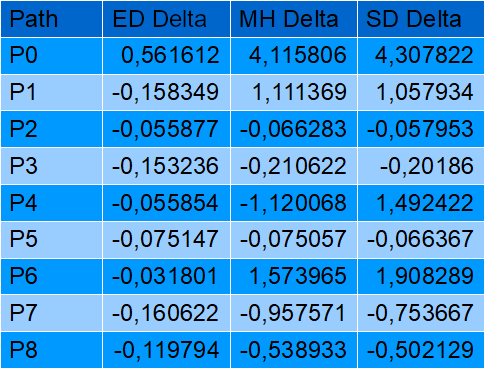
\includegraphics[width=0.5\textwidth,height=\textheight,keepaspectratio]{ChartsAndFigures/Edgy_timeTable.png}
\caption{Edgy Time Table}
Total time gain using waypoints in milliseconds.
\label{fig:Edgy_cd}
\end{figure}
In the smallest map, Edgy (Appendix~\ref{ap.edgy}), when the Euclidean Distance heuristic is used, it is cheaper to simply use raw A* directly on the grid to generate the path due to the added overhead when using waypoints. The other heuristics show no significant gain with waypoints added to the map, except the P0-path as seen in Figure~\ref{fig:Edgy_cd}, but this path is a worst case scenario.
	
While traversing the maps Edgy2 (Appendix~\ref{ap.edgy2}) and UMAP2 (Appendix~\ref{ap.umap2}), which are much greater in size compared to Edgy, the results shows that Waypoint traversal is superior to raw A* pathfinding. On almost all the paths tested, to traverse the waypoints first and direct the A*, gets a much smaller total time spent calculating the path. This proves that the waypoint traversal added are improving the total time spend calculating the path. Though the results show that in some cases using waypoints, the total time is increased compared with raw A*. This is because these paths are short or straight, with no or few blocked tiles in the way of the pathing.
	
In the comparison diagrams the color green, purple and red boxes represents traversal with waypoints with the Euclidian Distance- , Manhattan Distance- and Standford distance heuristic.
The color blue, cyan and brown colors represent traversal with raw A* tile traversal with the Euclidian Distance- , Manhattan Distance- and Standford distance heuristic.
The  X-axis is the nine different paths and the Y-axis is time in milliseconds spent calculating the path.
\begin{figure}[h!]
\centering
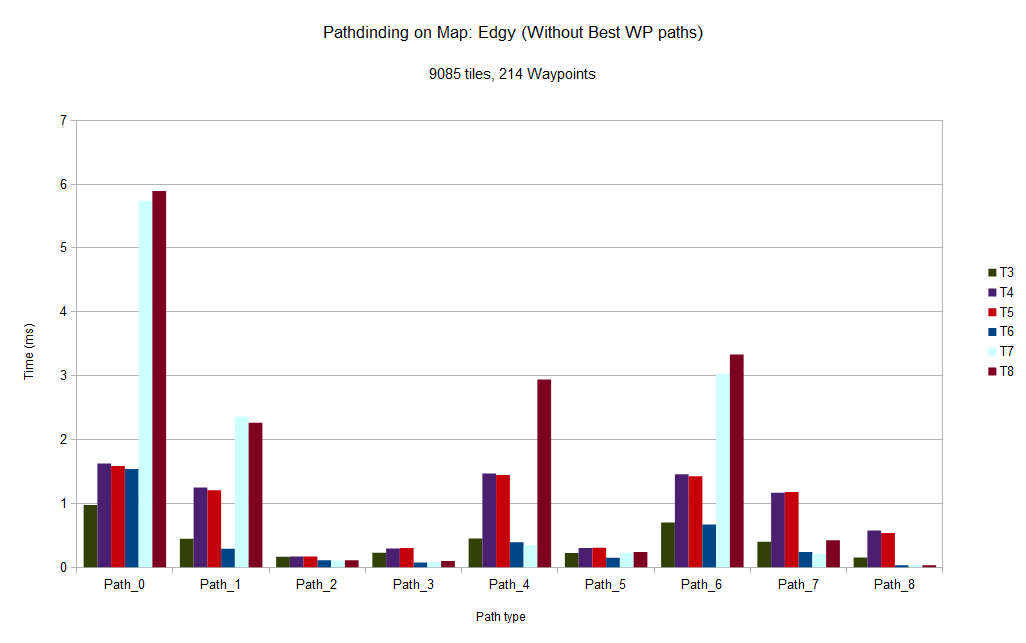
\includegraphics[width=0.5\textwidth,height=\textheight,keepaspectratio]{ChartsAndFigures/Edgy_d2.png}
\caption{Edgy Compare Diagram}
\label{fig:Edgy_d2}
\end{figure}	
On the map Edgy, in Figure \ref{fig:Edgy_d2}, we see all tests compared with each other. Its easy to see that in most cases, using only tile traversal is better than using the added waypoint traversal.
The average gain time can be seen in Figure \ref{fig:Edgy_cd} and in almost all cases the total time increases when traversing with waypoints.
	
However it is clearly displayed that waypoint traversal is superior to raw A* when the map size and complexity increases. Both Figure~\ref{fig:Edgy2_d2} and Figure~\ref{fig:UMAP2_d2} prove that the gain increases as the map grows.
Waypoint traversal was up to and above 40 milliseconds faster then raw A* pathfinding on UMAP2 and this is due to the maps edge case layout. In most cases the raw A* would get stuck in one of the U-shapes while searching for the goal, whereas the added waypoint traversal would quickly guide the A* to exit the rabbit hole and continue in the right direction. The exact avarge gain can be seen in Figure \ref{fig:Edgy2_cd} and Figure \ref{fig:UMAP2_cd}.
	
The validity of the experiments have a P value way below 0.05, mostly closely to 0.00.
\begin{figure}[h!]
\centering
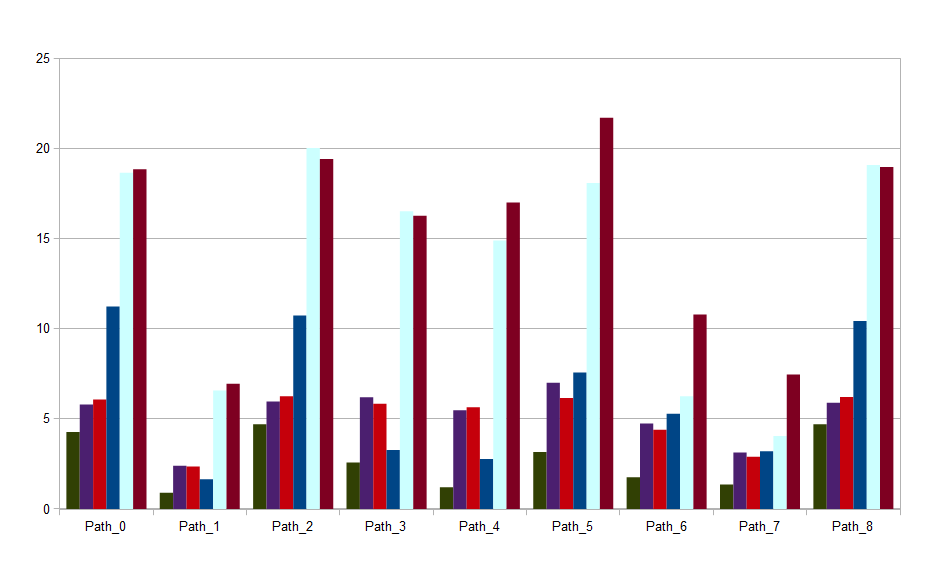
\includegraphics[width=0.5\textwidth,height=\textheight,keepaspectratio]{ChartsAndFigures/Edgy2_d2.png}
\caption{Edgy2 Compare Diagram}
\label{fig:Edgy2_d2}
\end{figure}
\begin{figure}[h!]
\centering
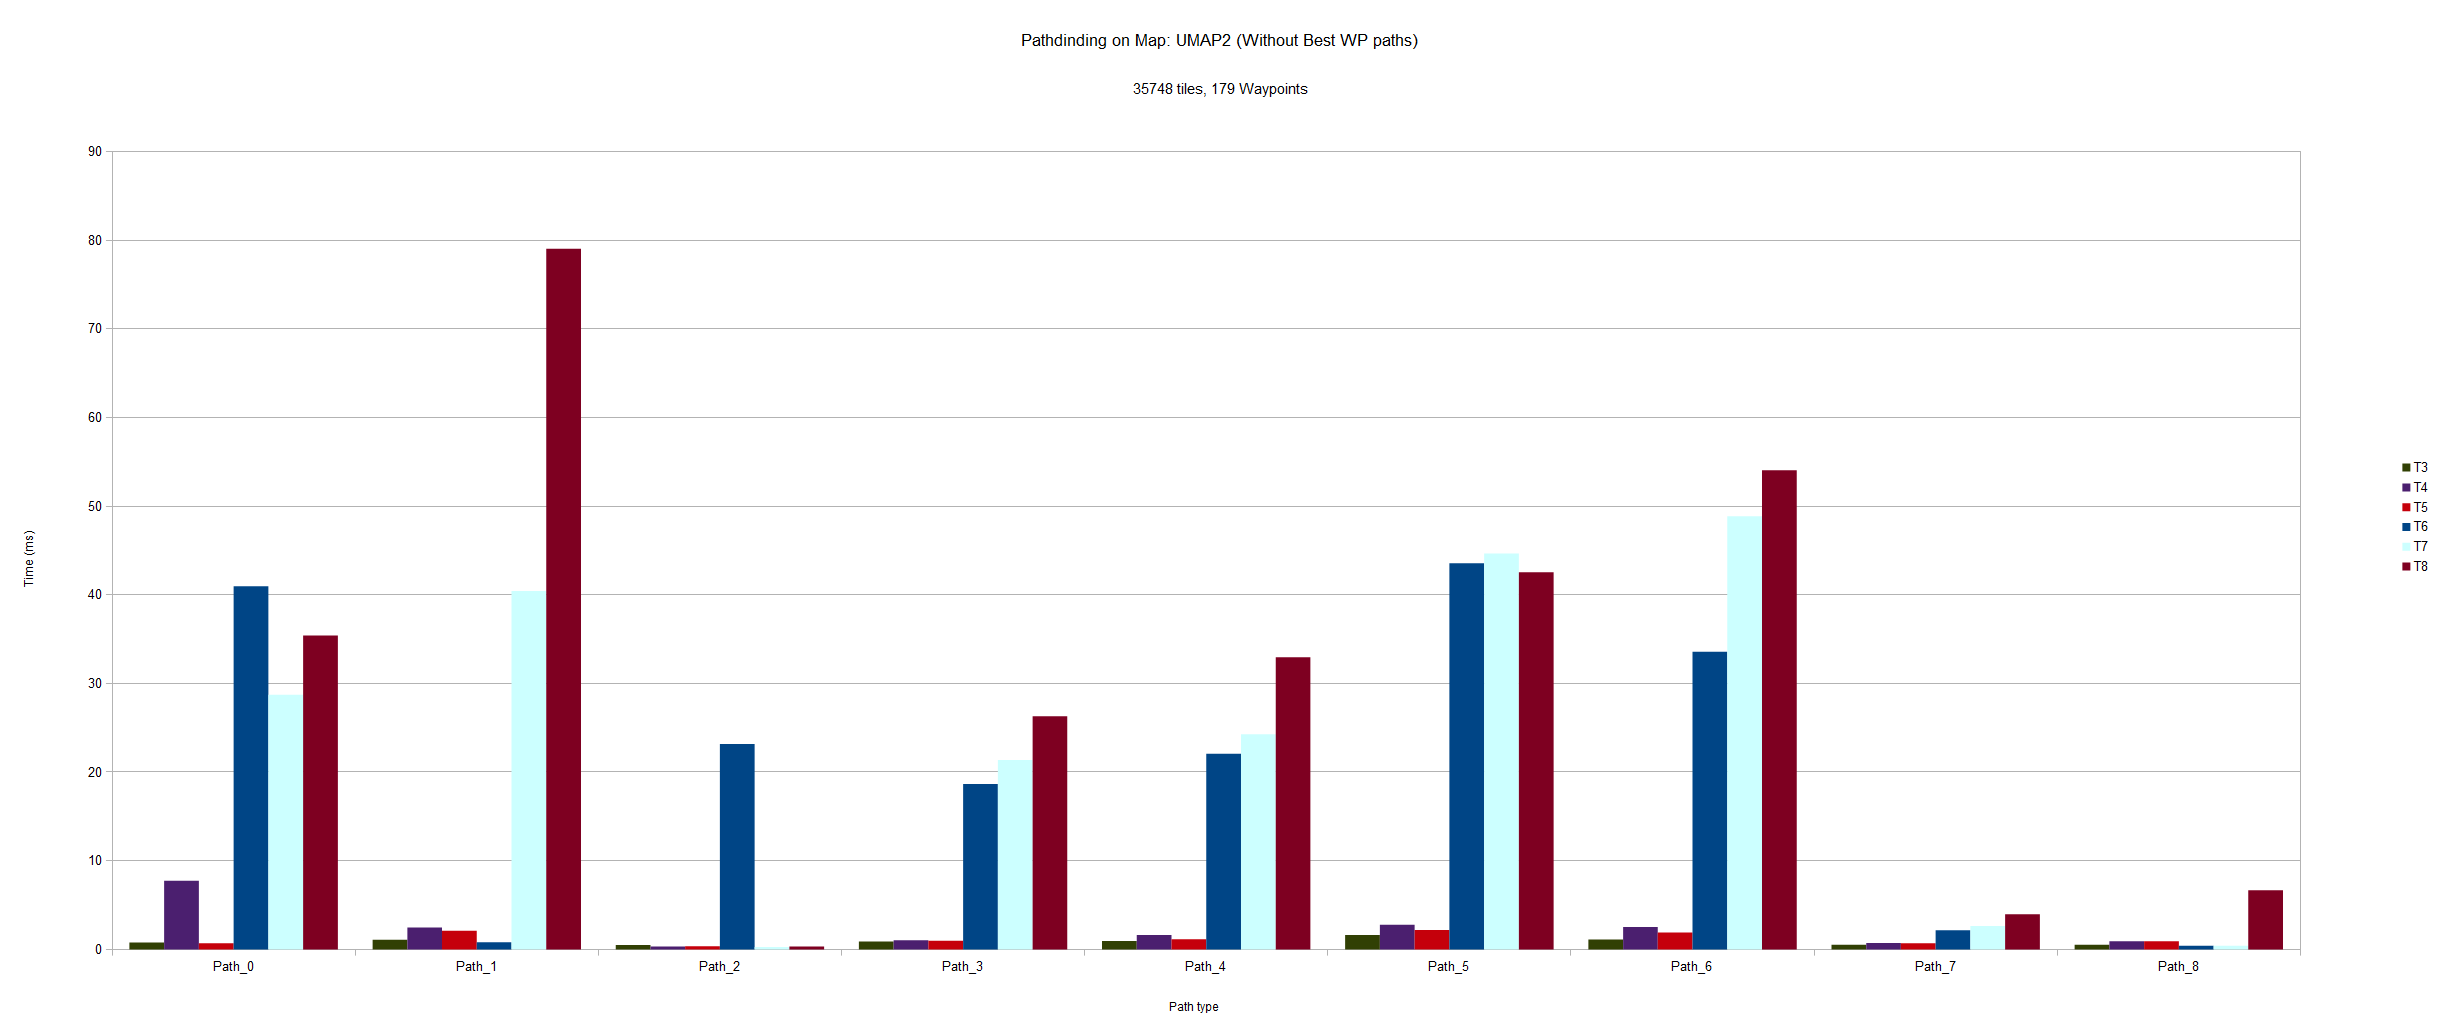
\includegraphics[width=0.5\textwidth,height=\textheight,keepaspectratio]{ChartsAndFigures/UMAP2_d2.png}
\caption{UMAP2 Compare Diagram}
\label{fig:UMAP2_d2}
\end{figure}
\begin{figure}[h!]
\centering
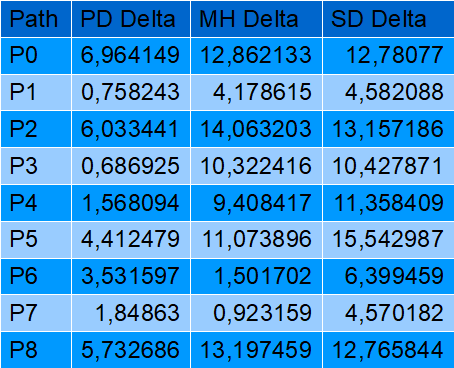
\includegraphics[width=0.5\textwidth,height=\textheight,keepaspectratio]{ChartsAndFigures/Edgy2_timeTable.png}
\caption{Edgy2 Time Table}
Total time gain using waypoints in milliseconds.
\label{fig:Edgy2_cd}
\end{figure}
\begin{figure}[h!]
\centering
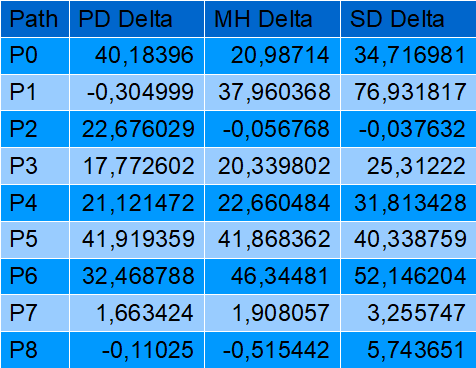
\includegraphics[width=0.5\textwidth,height=\textheight,keepaspectratio]{ChartsAndFigures/UMAP2_timeTable.png}
\caption{UMAP2 Time Table}
Total time gain using waypoints in milliseconds.
\label{fig:UMAP2_cd}
\end{figure}

\section{Conclusion and Future work}
On smaller maps with a lot of waypoint connections, raw A* is quicker than with our generation of waypoints. But when the map starts to scale, waypoints are significantly better than just A* by itself.
Our results are based on the first path the algorithm finds, not the quickest. In all our tests we also measured the time it took when using the quickest path for the waypoint traversal and this were proven to take more time than using raw A* with the first path found. It was only on UMAP2 we could get the quickest path for waypoints and still get less calculation time then just raw A*, but it were still not real time friendly. We got this result due to the real edge case layout of the map.
	
In the way the waypoints are generated there are no way of controlling how many there will be, it all depends of the complexity of the map. In future work there could be another approach of finding the waypoints based of the complexity of the map so that the average gain would always be positive.

\pagebreak
\begin{thebibliography}{9}

\bibitem{dynaPF15}
  Weiping Zhu, Daoyuan Jia, Hongyu Wan, Tuo Yang, Cheng Hu, Kechen Qin, Xiaohui Cui,
  \textit{Waypoint Graph Based Fast Pathfinding in Dynamic Environment},
  International Journal of Distributed Sensor Networks, vol. 2015, Article ID 238727, 12 pages,
  August 2015. https://doi.org/10.1155/2015/238727.

\bibitem{roboGame15}
  Zeyad Abd Algfoor, Mohd Shahrizal Sunar, Hoshang Kolivand,
  \textit{A Comprehensive Study on Pathfinding Techniques for Robotics and Video Games},
  International Journal of Computer Games Technology, vol. 2015, Article ID 736138, 11 pages,
  2015. https://doi.org/10.1155/2015/736138.

\bibitem{heuristicGame15}
  Geethu Elizebeth Mathew,
  \textit{Direction Based Heuristic For Pathfinding In Video Games},
  Procedia Computer Science, vol. 47, pp. 262-271,
  2015.

\bibitem{heuristicRef}
   Patel, Amit,
  \textit{Amit's Thoughts on Pathfinding},
  2019-02-22,
  http://theory.stanford.edu/~amitp/GameProgramming/Heuristics.html,
  (Accessed 2019-03-20).

%\bibitem{lamport94}
%  Leslie Lamport,
%  \textit{\LaTeX: a document preparation system},
%  Addison Wesley, Massachusetts,
%  2nd edition,
%  1994.

\end{thebibliography}


\clearpage
\onecolumn
\appendix
\appendixpage
\addappheadtotoc

\section{Map Edgy}\label{ap.edgy}
\centering
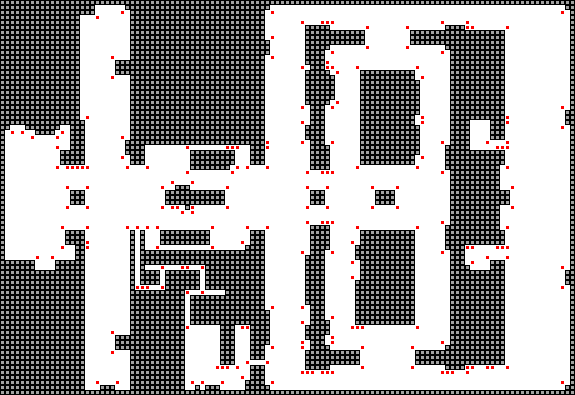
\includegraphics[width=\textwidth,height=\textheight,keepaspectratio]{ChartsAndFigures/Edgy.png}
9085 tiles, 4226 blocked (46.5\%). 214 waypoints with 2228 connections. Gray boxes indicates blocked tiles, Red boxes indicates waypoints and white space are open tiles.

\flushleft
\pagebreak
\section{Map Edgy2}\label{ap.edgy2}
\centering
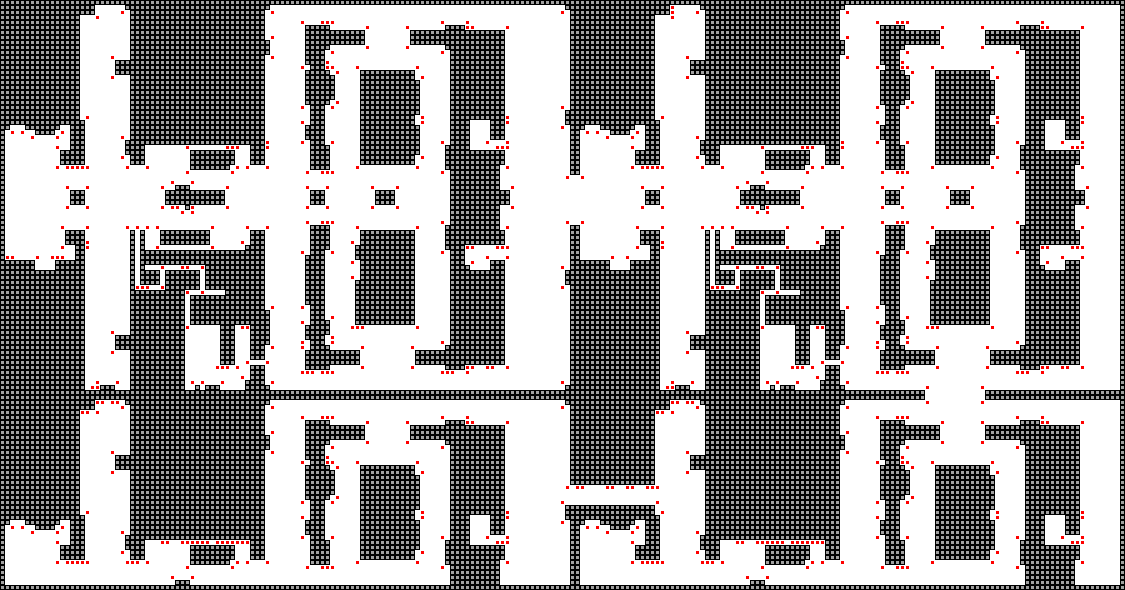
\includegraphics[width=\textwidth,height=\textheight,keepaspectratio]{ChartsAndFigures/Edgy2.png}
26550 tiles, 12854 blocked (48.4\%). 658 waypoints with 6458 connections. Gray boxes indicates blocked tiles, Red boxes indicates waypoints and white space are open tiles.

\flushleft
\section{Map UMAP2}\label{ap.umap2}
\centering
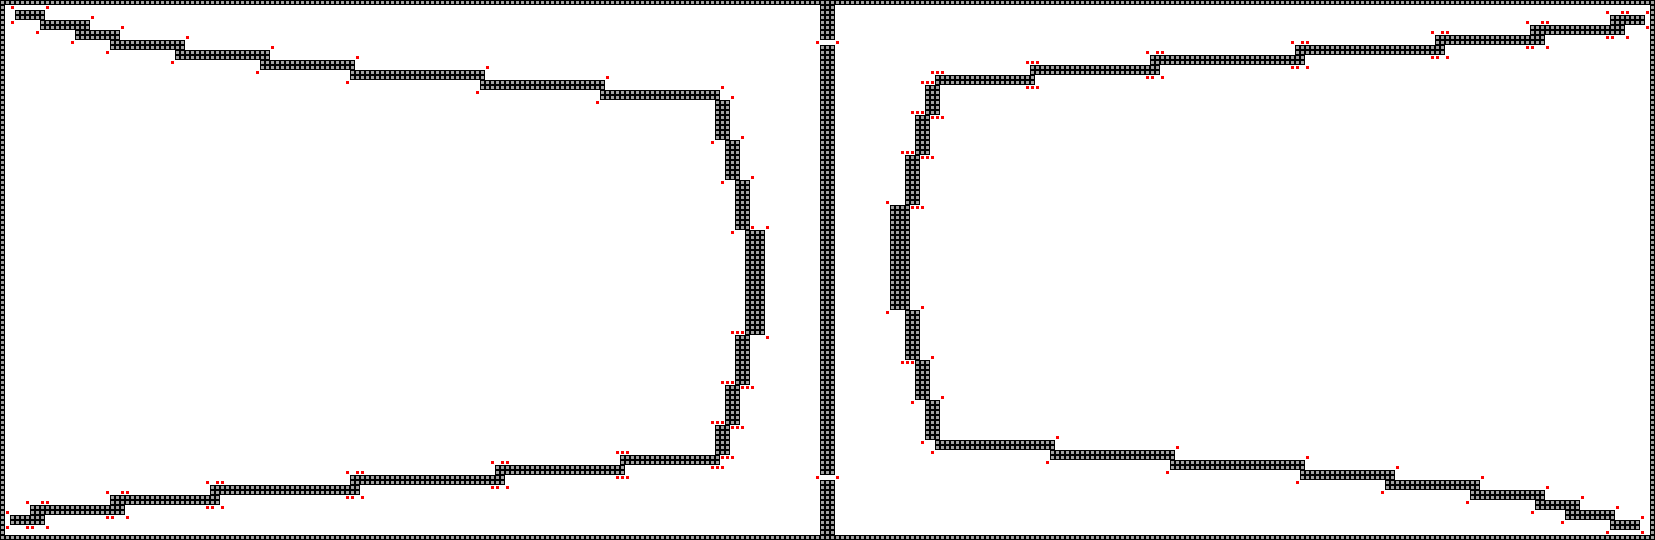
\includegraphics[width=\textwidth,height=\textheight,keepaspectratio]{ChartsAndFigures/UMAP2.png}
35748 tiles, 2890 blocked (8\%). 179 waypoints with 2038 connections. Gray boxes indicates blocked tiles, Red boxes indicates waypoints and white space are open tiles.


\end{document}
